\chapter{Implementação do protótipo conectado}
\label{cap:implementacao}
\rubricaFuncionalidade
\section{Materiais e implementação embarcada}\label{sec:bom}
O protótipo utiliza ESP32-D0WD-V3, sensor digital DHT11, visor SSD1306 de 0,96~pol, protoboard e cabos. Foi compilado com o pacote ESP32 da Arduino IDE, biblioteca Adafruit DHT, Adafruit SSD1306/GFX, ArduinoJson 7 e \texttt{arduino-mqtt} de Joel Gaehwiler. A alimentação foi realizada por USB/powerbank de acordo com a etapa experimental; não há acionamento elétrico de climatizador ou umidificador.
\subsection{Registro fotográfico do experimento}
As Fotografias~\ref{fig:foto-arranjo}, \ref{fig:foto-climatizador} e \ref{fig:foto-ar} documentam o arranjo físico utilizado na campanha, incluindo o nó IoT sobre protoboard, o computador empregado na programação e supervisão, o climatizador/umidificador portátil e o ar-condicionado de parede usados nas intervenções manuais. Essas imagens complementam os \emph{prints} de software e ajudam a caracterizar o ambiente experimental real em que a coleta foi executada.
\begin{figure}[H]
\centering
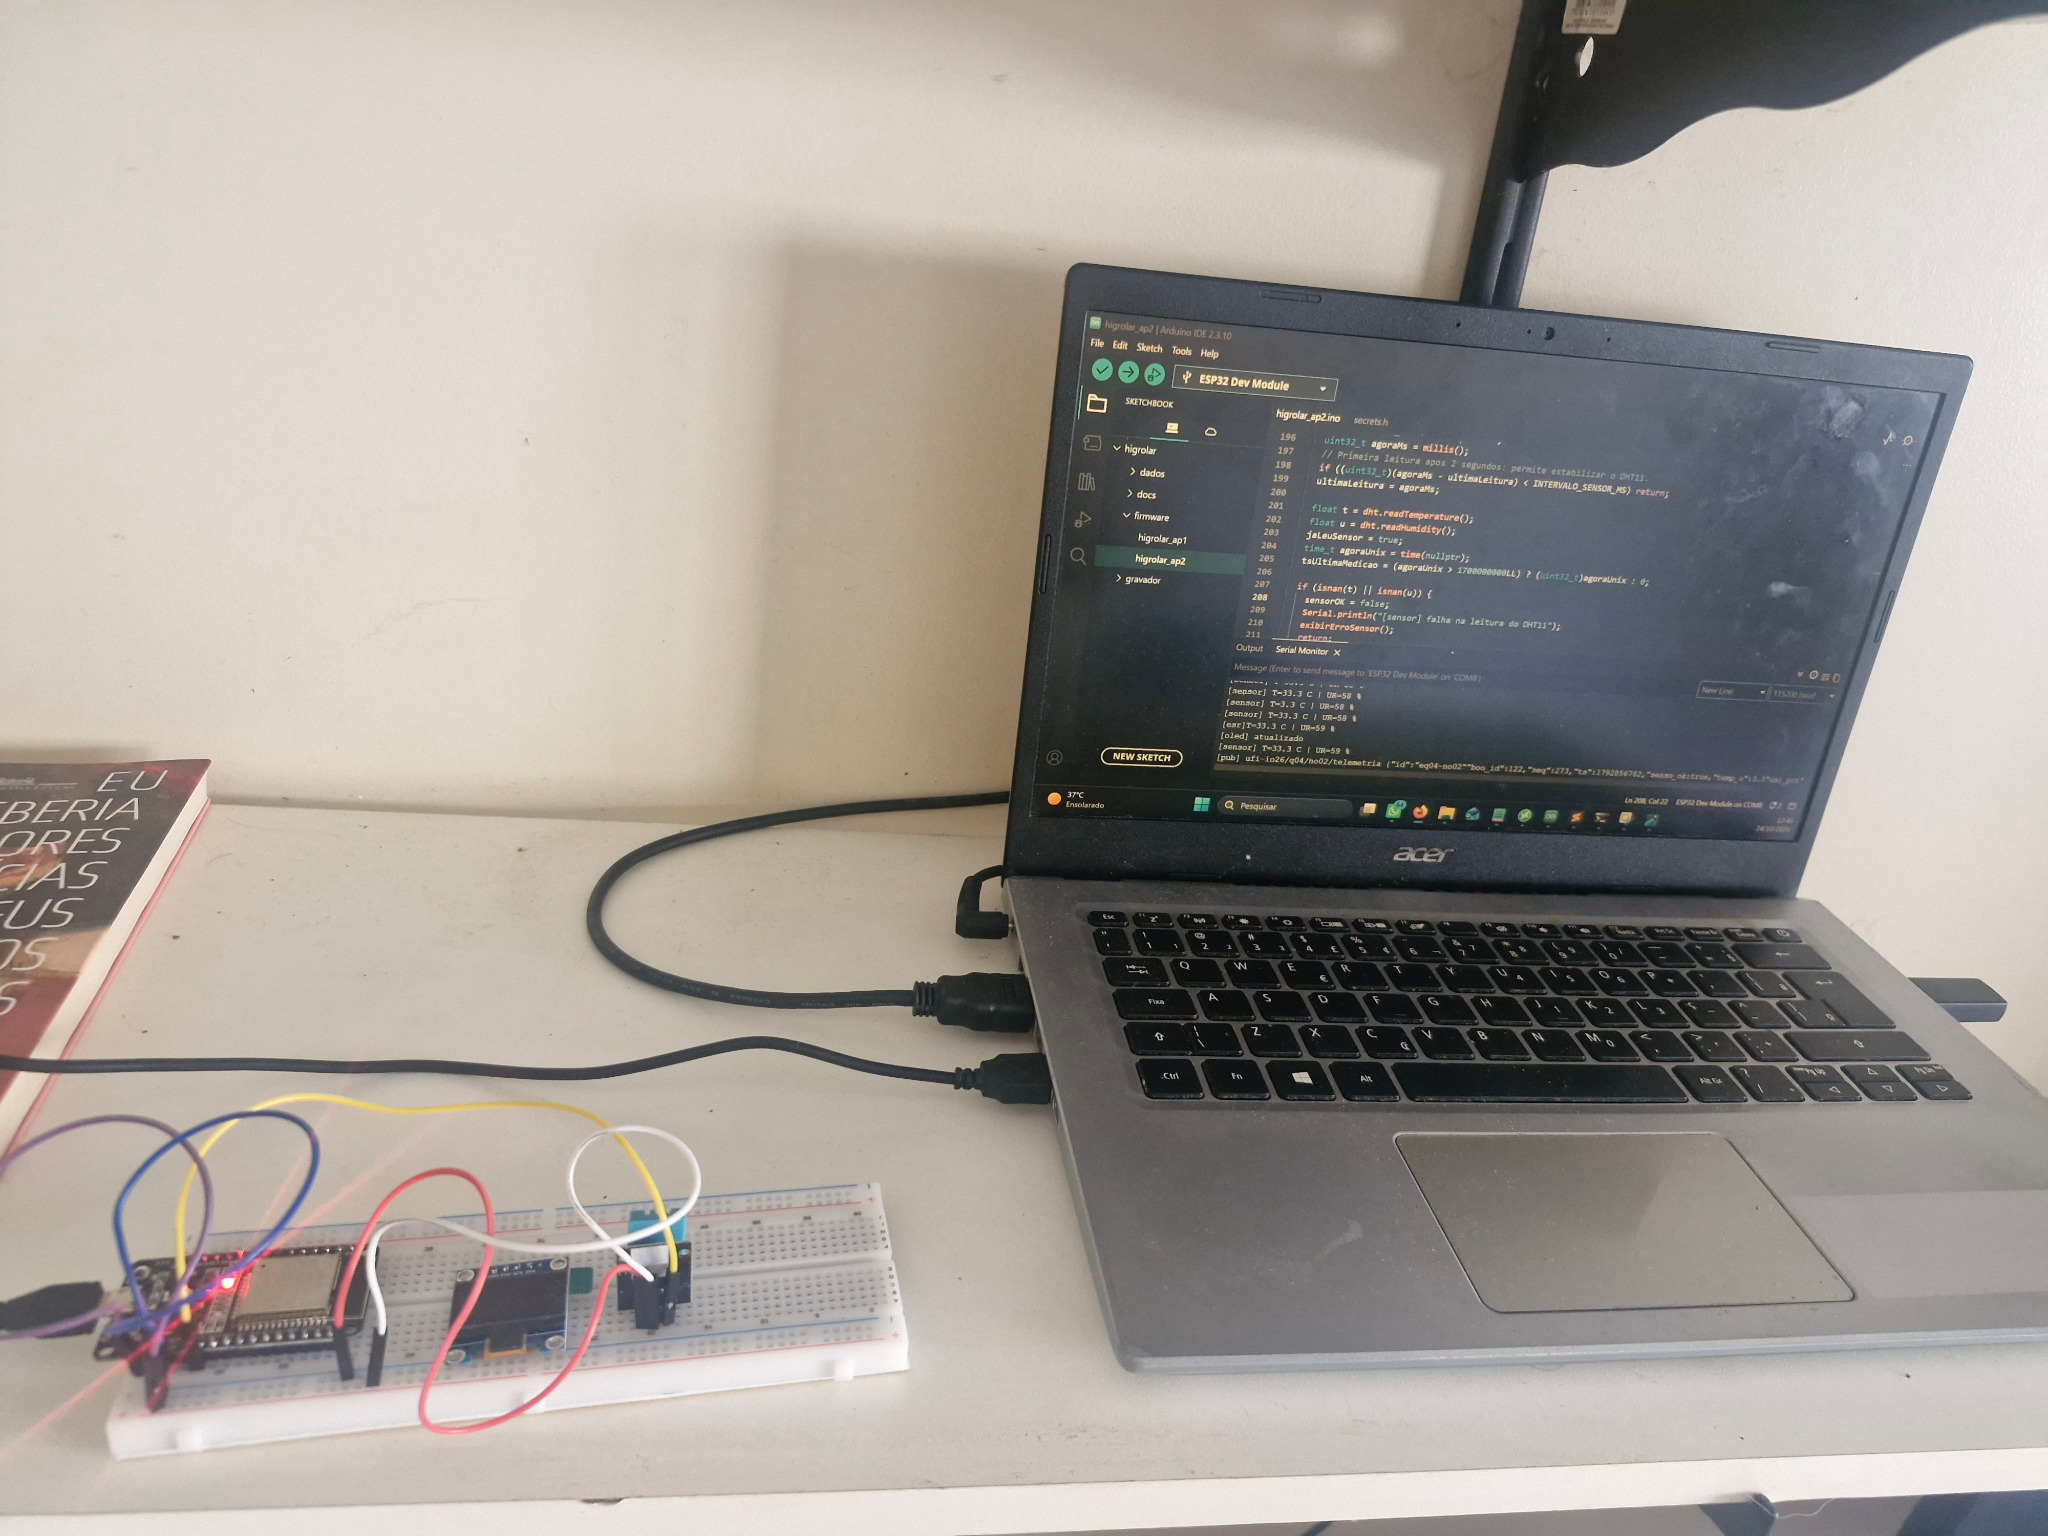
\includegraphics[width=.88\textwidth]{evidencias/fotos/arranjo_experimental.jpg}
\caption{Arranjo experimental de bancada com notebook, ESP32 em protoboard e periféricos usados na campanha.}
\label{fig:foto-arranjo}
\fonte{Fotografia da equipe, 24/10/2026.}
\end{figure}
\begin{figure}[H]
\centering
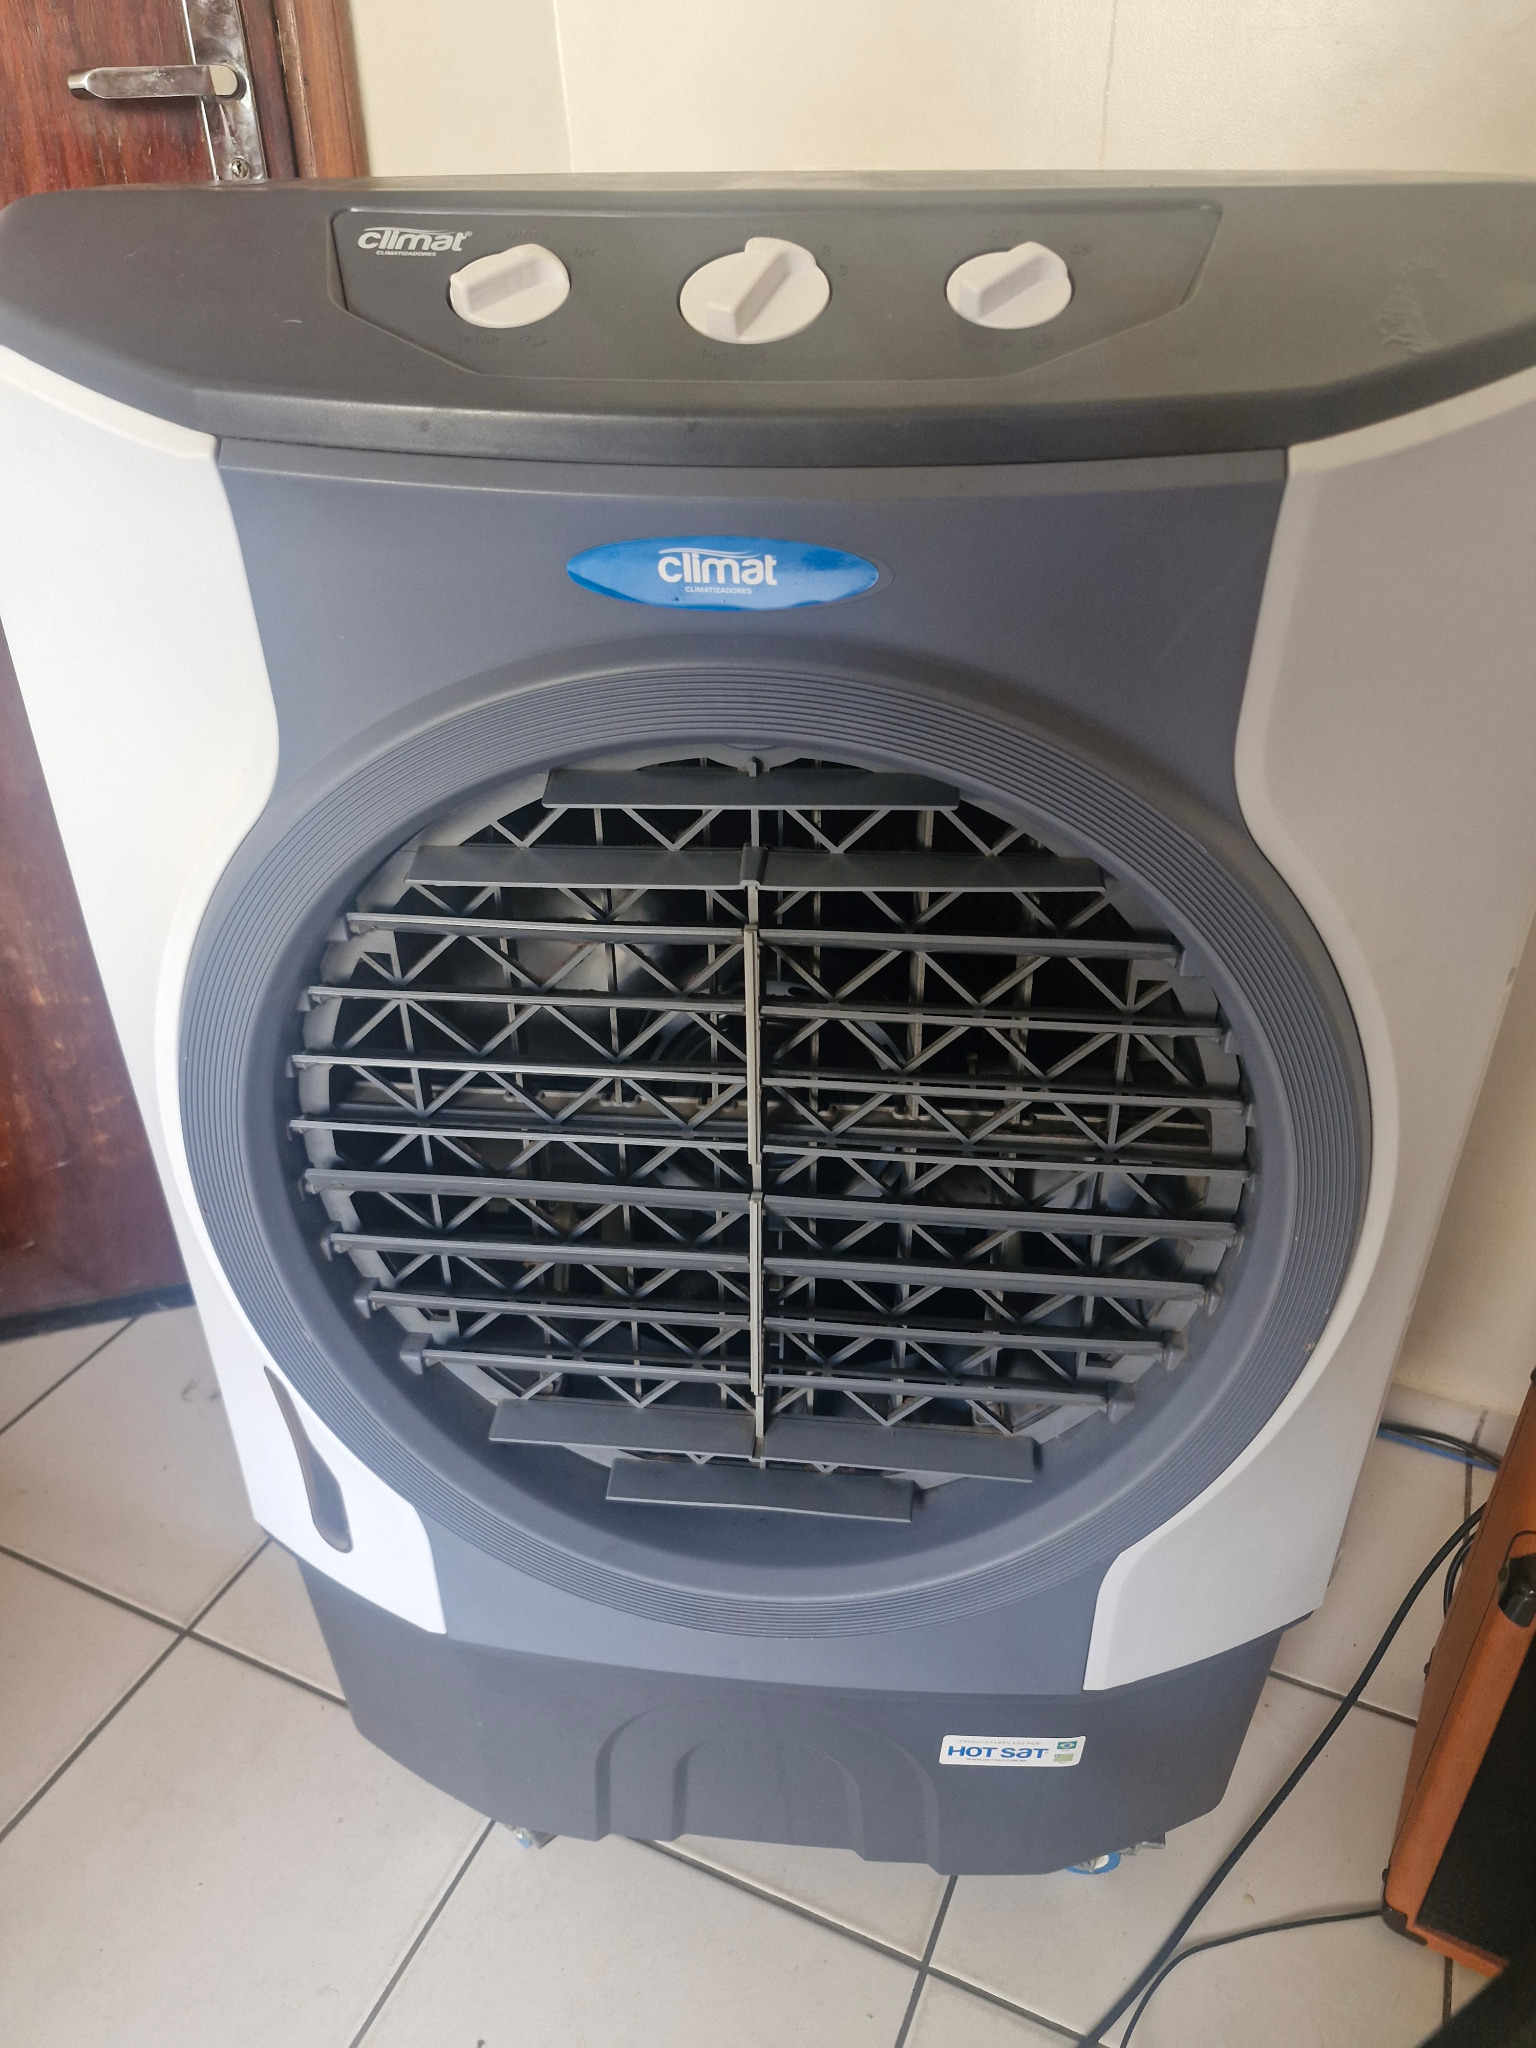
\includegraphics[width=.62\textwidth]{evidencias/fotos/climatizador.jpg}
\caption{Climatizador/umidificador portátil empregado nos ensaios de aumento de umidade e nos testes em operação simultânea.}
\label{fig:foto-climatizador}
\fonte{Fotografia da equipe, 24/10/2026.}
\end{figure}
\begin{figure}[H]
\centering
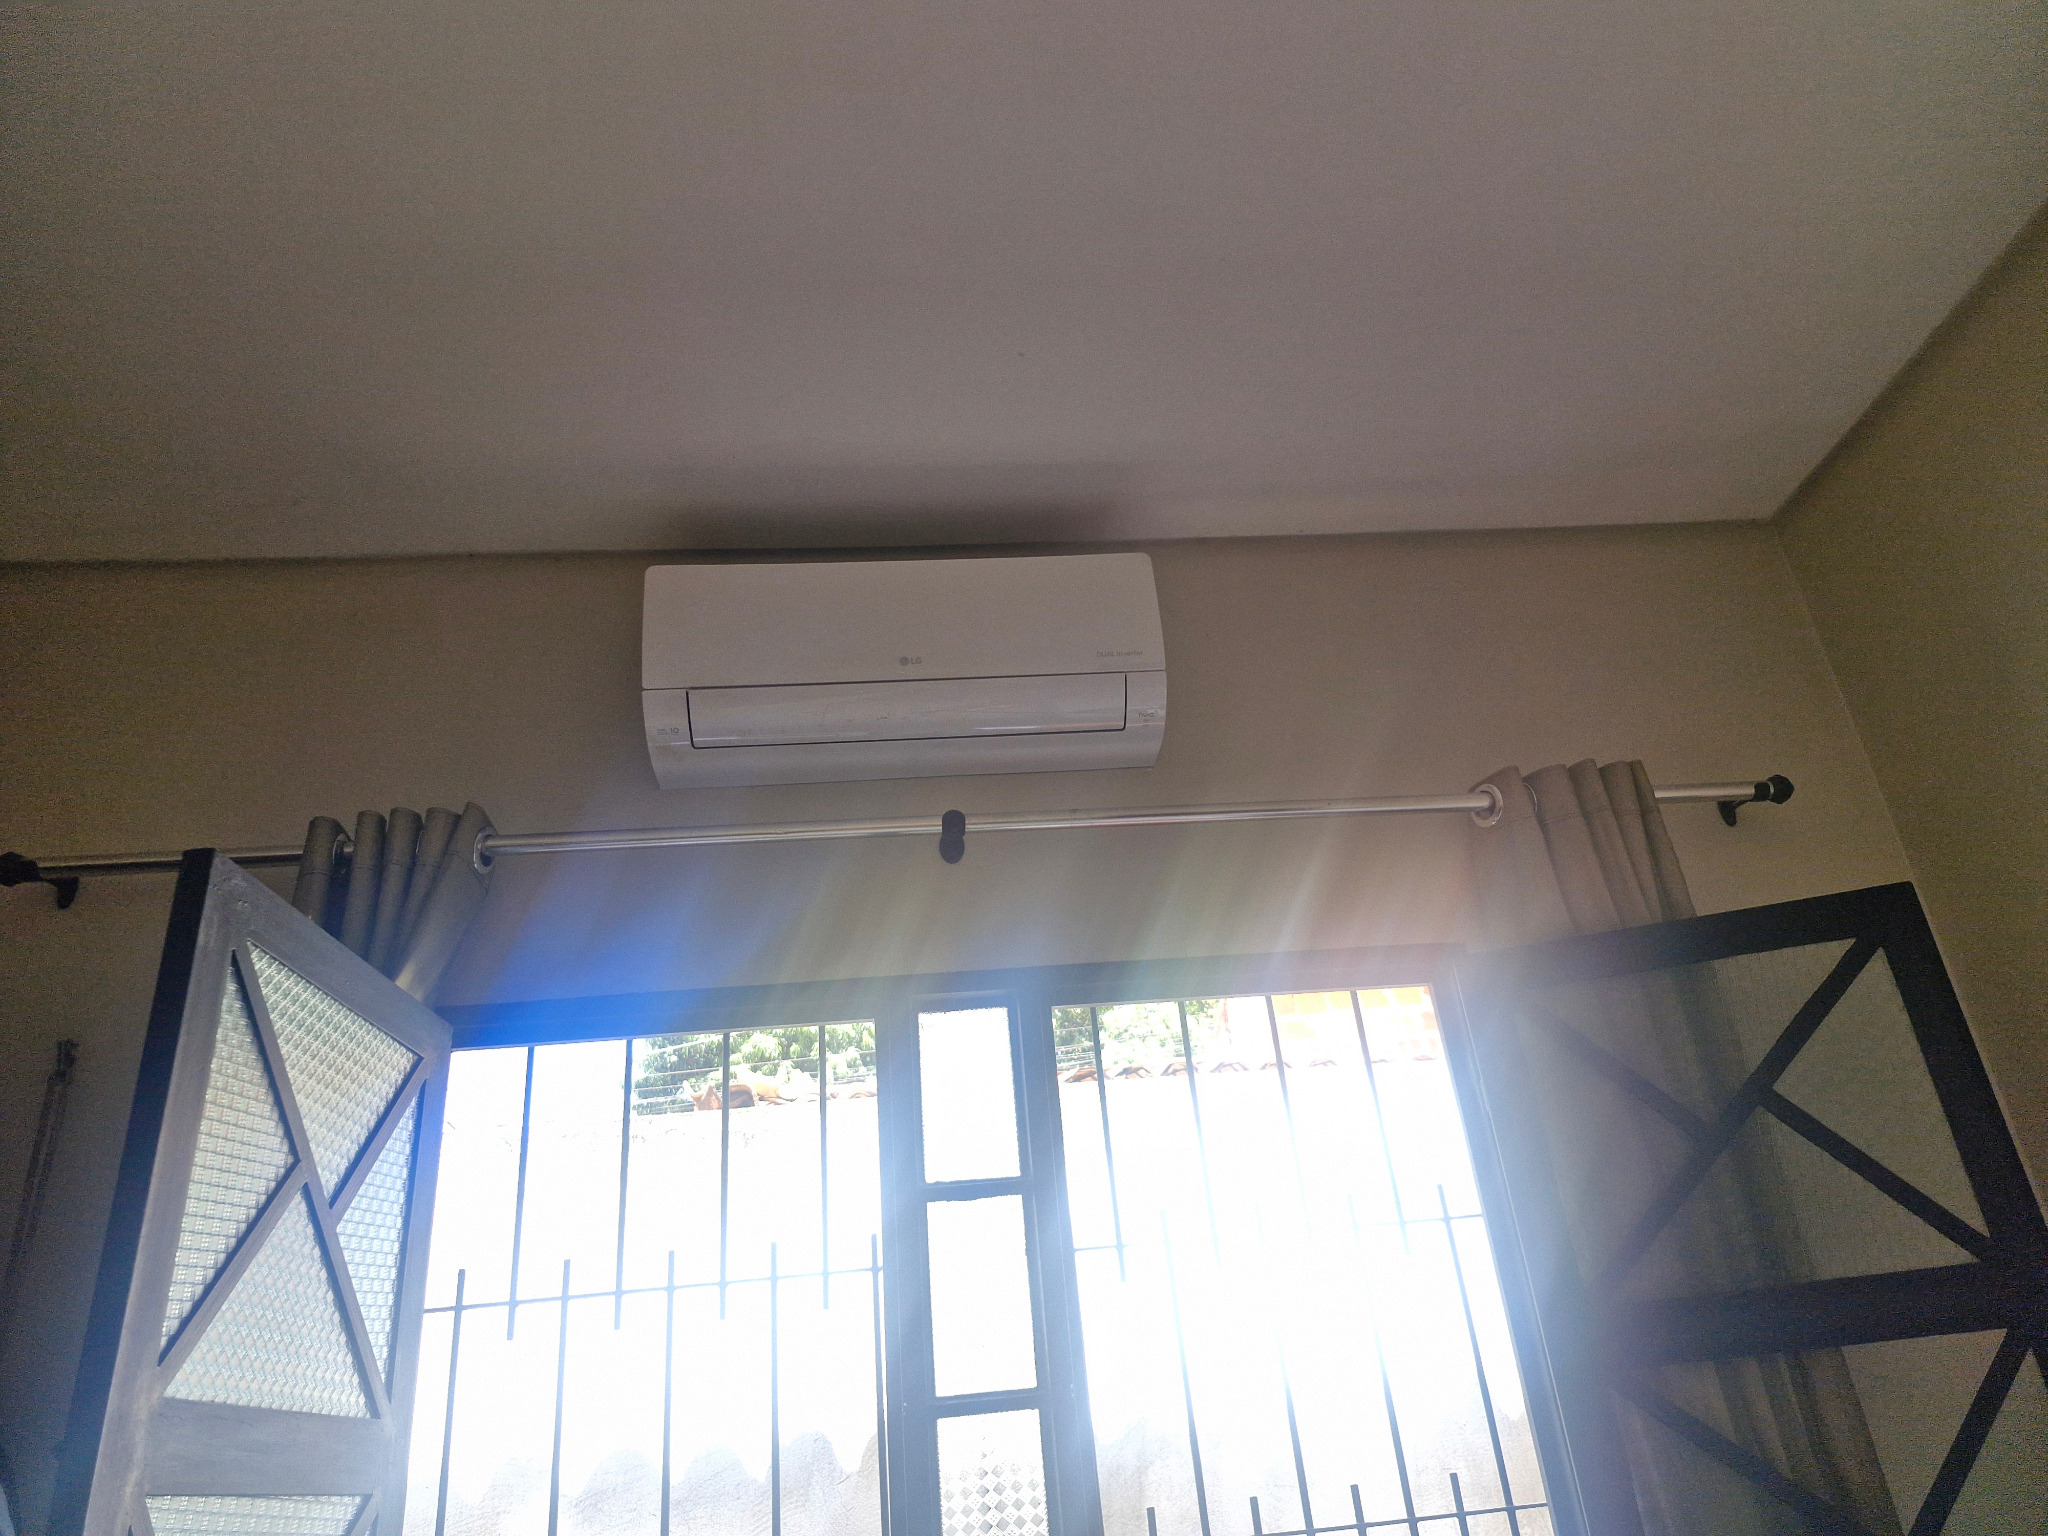
\includegraphics[width=.88\textwidth]{evidencias/fotos/ar_condicionado.jpg}
\caption{Ar-condicionado do ambiente, utilizado nos ensaios de refrigeração isolada e em conjunto com o umidificador.}
\label{fig:foto-ar}
\fonte{Fotografia da equipe, 24/10/2026.}
\end{figure}
\section{Leitura, comunicação e agendamento}\label{sec:firmware}
No \texttt{loop()}, cinco tarefas cooperativas executam leitura do sensor, conexão Wi-Fi, conexão MQTT, agendamento de telemetria e envio da fila, cedendo tempo com \texttt{delay(1)}. Os nomes reais das tarefas estão no código-fonte. O intervalo do sensor é 2~s. O intervalo de publicação inicia em 5~s e é configurado pelo tópico MQTT para 30~s na campanha. A serialização JSON acontece ao descarregar um item da fila; a captura da leitura e sua numeração ocorrem antes, inclusive sem rede.
\begin{lstlisting}[style=arduino,caption={Laço cooperativo do firmware de campanha},label={lst:laco}]
void loop() {
  tarefaSensor();
  tarefaWiFi();
  tarefaMQTT();
  tarefaAgendarTelemetria();
  tarefaEnviarFila();
  delay(1);
}
\end{lstlisting}
O ESP32 gera um contador de inicializações \texttt{boot\_id} salvo pela biblioteca \texttt{Preferences} na NVS. Cada amostra é identificada por \texttt{(id,boot\_id,seq)}; a variável \texttt{seq} reinicia a cada partida, mas o \texttt{boot\_id} muda. A fila circular tem capacidade máxima de 120 registros; quando lotada, o firmware descarta o mais antigo e incrementa a contagem de descartes. A publicação utiliza QoS 1; o retorno de sucesso do método de envio não equivale, por si só, a uma garantia de durabilidade ponta a ponta no CSV.
\section{Estados de conectividade}
A associação Wi-Fi é tentada no início e novamente depois de aproximadamente 15~s sem conexão. MQTT é retentado após 5~s; o assinante de configuração altera \texttt{periodo\_s} entre 2 e 3.600~s. O MQTT usa \emph{keepalive} de 30~s, publicação \texttt{online} retida e testamento \texttt{offline}. O relógio é inicializado por NTP; até haver horário válido o campo \texttt{ts} recebe \texttt{null}.
\section{Gravador, auditoria e rastreabilidade do código}
O \texttt{gravador.py} usa Paho-MQTT 2.x, MQTT 3.1.1 com TLS na porta 8883, sessão persistente e confirmação manual após escrita em CSV. Um certificado confiável é obtido do repositório de autoridades do Windows/sistema por \texttt{ssl.create\_default\_context}; há usuários distintos no EMQX para nó, visualização e gravador. O arquivo resultante preserva horário de recepção, tópico, \texttt{payload}, QoS, flag DUP e campos \texttt{id}, \texttt{boot\_id} e \texttt{seq}. A aplicação de qualidade calcula duplicações por chave composta e intervalos lacunosos por inicialização.
\par\noindent\textbf{Rastreabilidade Git:} o repositório organiza as fontes em \texttt{docs/}; \texttt{firmware/}, em que \texttt{higrolar\_ap2/} é a versão da campanha, com o modelo \texttt{secrets.example.h}; \texttt{gravador/}, com \texttt{gravador.py} e \texttt{qualidade.py}; e \texttt{dados/} (CSV bruto, \texttt{limpar.py} e o CSV limpo derivado dele). O CSV bruto da campanha entrou no \emph{commit} \texttt{e722db7} e não foi alterado depois.
\par\noindent Repositório: \url{\repositorioEquipe}\\
\emph{Commit} correspondente a esta entrega: o marcado pela \emph{tag} \texttt{ap2-final}.

\section{Gestão do broker EMQX e segregação de identidade}
A adaptação ao laboratório trocou o host HiveMQ de demonstração por uma instância EMQX Cloud, mantendo MQTT 3.1.1, QoS~1 e os três tópicos da equipe. As credenciais de autenticação são distintas: \texttt{higrolar-esp32} publica telemetria/status e assina configuração; \texttt{higrolar-monitor} assina a árvore e publica comandos de configuração; \texttt{higrolar-gravador} assina a árvore para persistir dados. Os \emph{client IDs} também são distintos. As permissões vistas no painel são documentadas na Seção~\ref{sec:topicos}; como a autorização estava em \emph{blacklist}, tais regras explícitas não garantem negação de operações não correspondentes. O gravador valida TLS no Windows, mas o nó utiliza \texttt{setInsecure()} quando não é informado um certificado CA. O arquivo \texttt{secrets.h} não integra o pacote de entrega.
